\section{Theorie\footnote{Unter Verwendung der Quellen \cite{demtroeder}, \cite{Versuchsanleitung} und \cite{gerthsen}.}}
\label{sec:Theorie}

Im folgenden Experiment soll die Abhängigkeit der dynamischen Viskosität von destilliertem Wasser untersucht werden. 
Hierfür wird auf die Kugelfall-Methode nach Ernst Fritz Höppler mit dem entsprechenden Viskosimeter zurückgegriffen, deren theoretische 
Grundlagen im Weiteren erläutert werden. 

\subsection{Strömungstypen und Viskosität}

Bewegt sich Flüssigkeit als Ganzes fort und finden nicht nur mikroskopische Bewegungen der einzelnen Teilchen innerhalb der 
Flüssigkeit statt, wird von einer Strömung gesprochen. 
Diese wird durch die Strömungsgeschwindigkeit ${\symbf{u}=\sfrac{\symup{d}\symbf{r}}{\symup{d}t}}$ eines am Ort $\symbf{r}$ 
zur Zeit $t$ befindlichen Teilchens beschrieben. 
Der dadurch festgelegte Weg $\symbf{r}(t)$ eines solchen Teilchens wird als \textbf{Stromlinie} beziehungsweise 
\textbf{Stromfaden} bezeichnet. 
Sie charakterisieren die Flüssigkeiten in ihrem Strömungsverhalten und werden unter anderem von den stattfindenden 
Reibungsverlusten innerhalb der Flüssigkeit oder zwischen zwei verschiedenen Medien beeinflusst. 
Die sogenannte Viskosität\footnote{Ist von Viskosität die Rede, ist meist die dynamische Viskosität gemeint. Es gibt ebenfalls 
die kinematische Viskosität $\nu$. Wenn diese erwähnt werden soll, wird dies üblicherweise ohne Weglassung des Attributs \textit{kinematisch} getan.} 
$\eta$ ist ein Maß für die Stärke der Reibung innerhalb des Mediums und hat die Einheit 
${\sfrac{\si{\newton\second}}{\si{\meter\squared}}=\si{\pascal\second}}$. 
Sie hängt unter anderem vom Stoff als auch von der Temperatur ab. 

Von Interesse seien hier vor allem viskose Flüssigkeiten. Nicht-viskose Flüssigkeiten -- auch \textbf{ideale Flüssigkeiten} 
-- haben eine Viskosität von ${\eta \approx 0}$, die innere Reibung ist bei diesen also vernachlässigbar klein. 
Strömungen viskoser Flüssigkeiten lassen sich in \textbf{laminare} und \textbf{turbulente Strömungen} unterteilen. 
Charakteristisch für eine laminare Strömung sind die durch die Stromlinien getrennten Flüssigkeitsschichten, die sich nicht miteinander vermengen. 
Hier überwiegt die innere Reibung der an den Randschichten. 
Ist dies nicht der Fall, destabilisiert sich diese Strömung und geht in eine turbulente über, bei der sich Wirbel und Ähnliches 
ausbilden. 
Besonders anschaulich wird dieser Sachverhalt unter Betrachtung der Abbildungen \ref{fig:lamturb} \subref{fig:laminar} und \subref{fig:turbo}. 

\begin{figure}
    \centering
    \begin{subfigure}{0.48\textwidth}
        \centering
        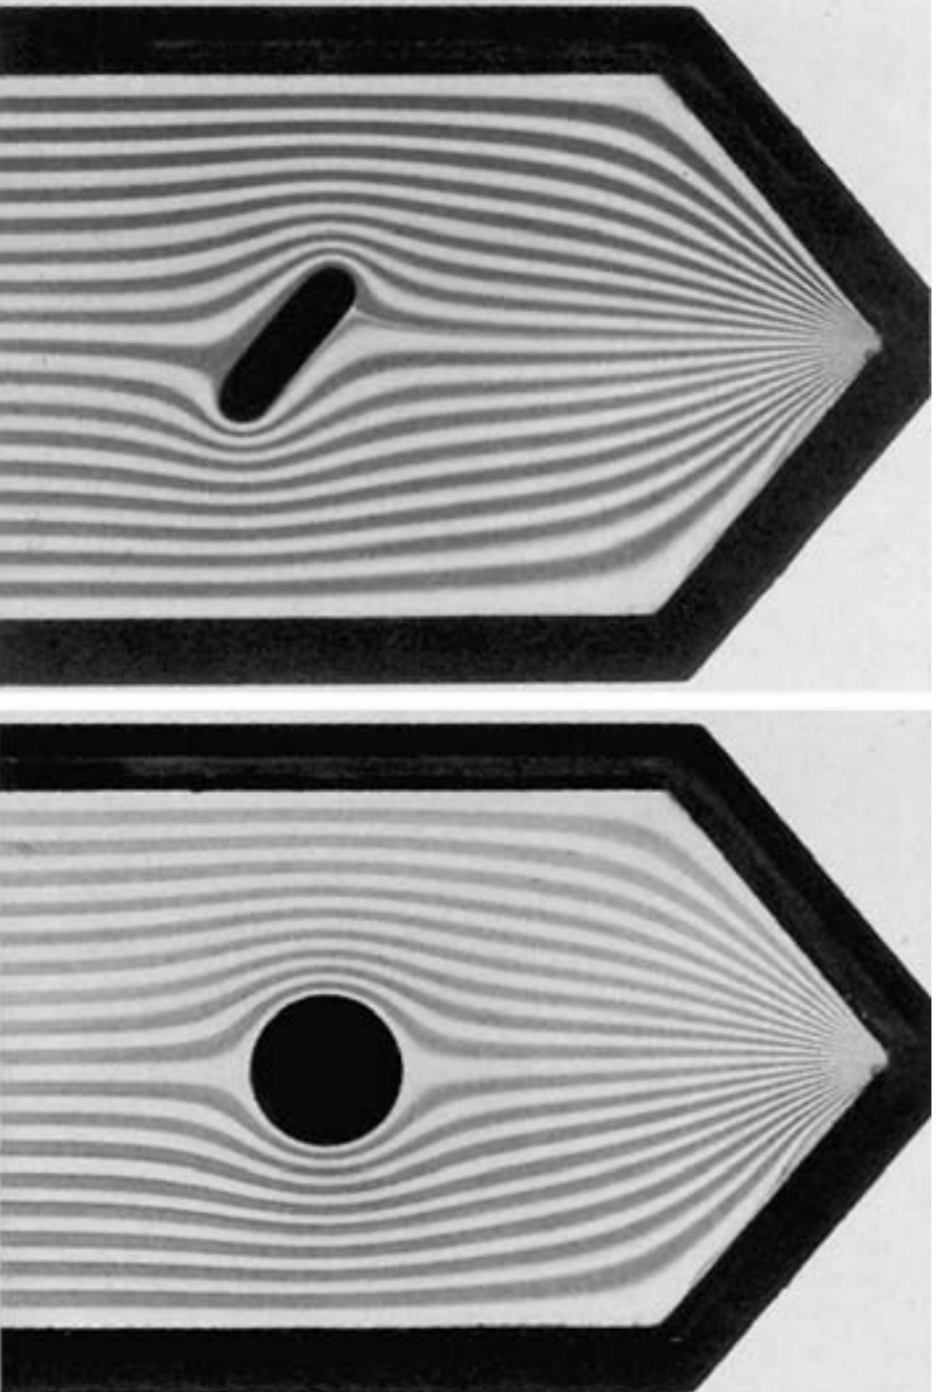
\includegraphics[height=6.75cm]{plots/demtr2.jpeg}
        \caption{Eine laminare Strömung\protect\cite{demtroeder}.}
        \label{fig:laminar}
    \end{subfigure}
    \begin{subfigure}{0.48\textwidth}
        \centering
        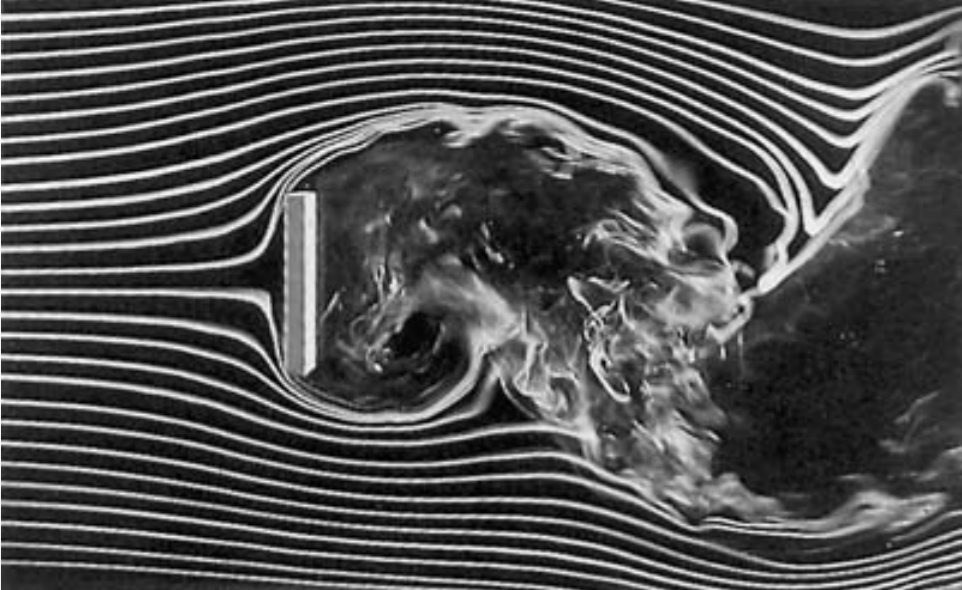
\includegraphics[height=4.75cm]{plots/demtr1.jpeg}
        \caption{Eine turbulente Strömung\protect\cite{demtroeder}.}
        \label{fig:turbo}
    \end{subfigure}
    \caption{Von links nach rechts laufende Strömungen viskoser Flüssigkeiten.}
    \label{fig:lamturb}
\end{figure}

Mithilfe der dimensionslosen \textbf{Reynoldszahl} $Re$ kann quantifiziert werden, inwieweit eine Flüssigkeit laminar beziehungsweise 
turbulent ist. 
Liegt $Re$ unterhalb der sogenannten \textbf{kritischen Reynoldszahl} $Re_c$, ist die Strömung laminar, ansonsten turbulent. 
Berechnet wird die Reynoldszahl über
\begin{equation}
    Re=\frac{\rho v L}{\eta} \:,
    \label{eqn:reynold}
\end{equation} 
wobei $\rho$ die Dichte der Flüssigkeit ist, $v$ die Geschwindigkeit eines Körpers gegenüber der Flüssigkeit und $L$ eine 
zu definierende charakteristische Länge, die der Geometrie der Situation entspricht. 
Ohne \ref{sub:hoppla} etwas vorwegzunehmen sei an dieser Stelle angemerkt, dass bei zylinderförmigen Behältern und kugelförmigen 
Fallkörpern, deren Durchmesser nur um Weniges kleiner sind als der des Zylinders, der Durchmesser $d$ häufig als $L$ gewählt wird. 

\FloatBarrier 

\subsection{Das Kugelfallviskosimeter nach Höppler}
\label{sub:hoppla}

Ein Kugelfallviskosimeter besteht aus einem zylinderförmigen Behälter, der mit vorzugsweise Wasser gefüllt. 
Darin befindet sich eine Röhre, die mit dem Fluid gefüllt wird, dessen Viskosität untersucht werden soll.
Über ein angeschlossenes Thermostat kann die Temperatur des Wassers reguliert werden, welche sich nach kurzer Zeit auf 
das Fluid überträgt. 
Das Prinzip beruht auf der \textit{Stokes'schen Reibung} $F_R$, die durch eine fallende Kugel im Fluid erzeugt wird. 
Quantifizieren lässt sich dies über 
\begin{equation}
    F_R = 6 \symup{\pi} \eta v r \:,
    \label{eqn:stokes}
\end{equation}
wobei $v$ die Geschwindigkeit und $r$ den Radius der Kugel darstellen. 
Ebenfalls der Gewichtskraft ${F_G = m\symup{g}}$ entgegen wirkt die Auftriebskraft 
\begin{equation}
    F_A = V \rho _\text{Fl} \symup{g} 
    \label{eqn:archimedes}
\end{equation}
mit dem durch die Kugel verdrängten Volumen $V$, der Dichte der Flüssigkeit $\rho _\text{Fl}$ und der Erdbeschleunigung $\symup{g}$. 

Wird eine Kugel am oberen Ende der Röhre in das Fluid gelassen, stellt sich nach kurzer Zeit ein Kräftegleichgewicht 
und dementsprechend eine gleichförmige Bewegung mit konstanter Geschwindigkeit ein. 
Aus dem Gleichgewicht 
\begin{equation}
    F_A + F_R = F_G
    \label{eqn:fix} %fix für Fixpunkt=>Gleichgewicht ;)
\end{equation}
lässt sich die dynamische Viskosität $\eta$ des Fluids bestimmen.
Daraus ergibt sich der Zusammenhang 
\begin{equation}
    \eta = K (\rho _\text{Körper} - \rho _\text{Fl}) t \quad \text{mit der Fallzeit} \: t.
    \label{eqn:exp_visk}
\end{equation}
Die Besonderheiten der spezifischen Apparatur, wie beispielsweise die Neigung der Röhre, werden mit der Konstante $K$ berücksichtigt. 

Da beim Kugelfallviskosimeter nach Höppler der innere Zylinder nur minimal größer als der Kugeldurchmesser ist, 
ist die Apparatur um wenige Grade geneigt, damit die Kugel nicht frei im Fluid herabsinkt, sondern an der Rohrinnenwand 
herabgleiten kann. 
Dies ist wichtig, um keine Turbulenzen beziehungsweise Wirbel zu erzeugen, da die Kugel sonst mehrere Male an die Wand stößt. 
Die Turbulenzen würden die Messergebnisse erheblich verfälschen. 

Das Vorgehen wird unter Variation der Temperatur mithilfe des genannten Thermostats durchgeführt, um eine Relation zwischen 
Temperatur und Viskosität herstellen zu können. 
Der Zusammenhang wird über die Andrade'sche Gleichung 
\begin{equation}
    \eta = A \symup{e}^{\frac{B}{T}}
    \label{eqn:andrade}
\end{equation}
mit den konstanten Parametern $A$ und $B$ und der Temperatur $T$ des Fluids hergestellt. 
